% Chapter Template

\chapter{Process} % Main chapter title

\label{Appendix D} % Change X to a consecutive number; for referencing this chapter elsewhere, use \ref{ChapterX}

%----------------------------------------------------------------------------------------
%	SECTION 1
%----------------------------------------------------------------------------------------

\section{Introduction}
This appendix elaborates on the process behind the development of the final product.

The project was initiated by the case presented by Struct A/S. The core of the case was as follows:
\textit{"When launching sites, whether it being regular websites or web shops, a lot of user activity is logged. We therefore have a large amount of data associated with each of our sites but do not currently use it.} \\
\textit{In the future we would like to be able to use logged data to generate an insight into the user activity on our site and actively use this data to create a personalized experience for the users."} \\
Eventually this case led to the problem statement seen in chapter \ref{chapter1_ProblemStatement}.

A variety of technologies and methods was used throughout the realization of the product. To ensure that the process went as smooth as possible, the agile software development framework, Scrum, was used as a framework to structure and organize the work \cite{Scrum}.

\section{Scrum}
Scrum is the main pillar for controlling the process of the project. Since the developing team only consisted of two students, Scrum is not applied 100\% to the project. This section elaborates on the usage of Scrum and how the different roles were fulfilled.

\subsection{Product owner}
The product owner is typically in charge of which tasks needs to be done in what order. He is in charge of the product backlog and ensures that the developing team keeps adding value to the final product. Since there was no product owner in this project, the role is carried out by the team itself together with the company. The project group kept track of the backlog and had regular feedback from Struct, to ensure the development was on the right track.

\subsection{Scrum master}
The scrum master has the responsibility of removing impediments to the development team, and ensures that the scrum framework is followed. No actual scrum master was elected, which means that the development team along with our supervisor took on the role.

\subsection{Workflow}
Sprints of the length two weeks were chosen, as this was a fitting amount of time to develop and gain feedback. The sprint backlog was filled with issues and prepared before every the start of each sprint. Every work day started with a scrum meeting, where todays work was discussed. At the end of each sprint a meeting was set up with the customer (Struct A/S) to present what was implemented to ensure the project was still on the right track. The sprint backlog for the next iteration was presented as well, and then adjusted according to any feedback from the customer.
By following these two week sprints, the project never deviated much from the wishes of the customer.


\section{GitHub}
The implementation of the final product required the usage of different tools. Github made it possible to structure and organize the planning, implementation and deployment of the project.\\

Git is a popular version control system and it is often used when developing software. GitHub is a web-based Git, and served as the primary tool when planning and developing the system. All planning is documented through GitHub issues and milestones. At the initial start, all project tasks was put in the product backlog which was made of issues. The sprints was created as milestones which was filled with issues before each iteration.
The implementation of the system was controlled with Git. A consistent way of using the tool ensured that the newest version of the system was always available to the other group member, and a roleback was always possible had it been necessary. The newest version of the system was always to be found on the \textit{master} branch. When adding new code, the group members had to create a new branch from the \textit{master} branch, to avoid conflicts later. Once the new code was added in its own branch, and tested to ensure there were no flaws, it was merged into the newest version of the \textit{master} branch.
Besides making it possible to work simultaneously on the project, GitHub also served as a backup of the entire project.

\color{red}\section{Initial data dump}
In the beginning of the project data from one of \gls{Struct}' customers was supplied. This data was in the form of many SQL tables and most of the data was not relevant for creating product recommendations. The main tables used were the following:  \\
\begin{itemize}
	\item Visitor: A collection of every unique visitor who had visited the customer's website, each visitor gets a unique identifier called UID. Contains 3,073,665  visitors.
	\item Profile: A collection of every users signed up at the website. Contains 3037 profiles.
	\item BehaviorData: A collection of every unique action performed by visitors on the website, for example when a visitor views a product a new row is made with the visitor's UID, the product UID and the timestamp. Contains 3,326,736 visitor actions.
	\item Order: Contains each profile's orders. Contains 5520 orders.
	\item Product: A collection of all products on the website with their unique IDs. Contains 22,445 products.
	\item ProductGroup: A collection of all product groups. Contains 262 product groups.
	\item AttributeValueRendered: A collection of product and product group descriptions in different languages. Contains 409,259 descriptions:
	
\end{itemize}

A snapshot of the visitor and behaviorData table can be seen in figure \ref{visitorTable} and \ref{behaviorTable}.

\begin{figure}[H]
	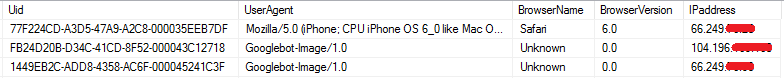
\includegraphics[scale=0.8]{Visitor_table}
	\caption{Visitor table from the original data}
	\label{visitorTable}
\end{figure}
\begin{figure}[H]
	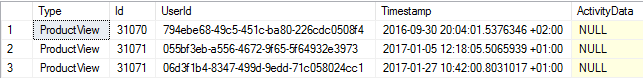
\includegraphics{behaviorData_table}
	\caption{Behavior data table from the original data}
	\label{behaviorTable}
\end{figure}

These tables contain all the pertinent information for creating product recommendations and can be utilized after a cleaning and structuring process. This process is described in the following sections.
